\documentclass[a4paper,12pt]{article}

\usepackage{float}

\usepackage[utf8]{inputenc}
\usepackage[dvips]{graphicx}
%\usepackage{a4wide}
\usepackage{epsfig}
\usepackage{fancybox}
\usepackage{verbatim}
\usepackage{array}
\usepackage{latexsym}
\usepackage{alltt}
\usepackage{amssymb}
\usepackage{amsmath,amsthm}
\usepackage{bm}
\usepackage{wasysym}

%\usepackage{fullpage}
%\usepackage{hyperref}
\usepackage{listings}
\usepackage{color}
\usepackage{algorithm}
\usepackage{algpseudocode}
\usepackage[hmargin=2cm,vmargin=3.0cm]{geometry}
%\topmargin=0cm
%\topmargin=-1.8cm
%\addtolength{\textheight}{6.5cm}
%\addtolength{\textwidth}{2.0cm}
%\setlength{\leftmargin}{-3cm}
%\setlength{\oddsidemargin}{0.0cm}
%\setlength{\evensidemargin}{0.0cm}

%misc libraries goes here
\usepackage{tikz}
\usepackage{tikz-qtree}
\usetikzlibrary{automata,positioning}

\usepackage{multicol}
\usepackage{enumitem}

\usepackage[most]{tcolorbox}

\usepackage[colorlinks=true,urlcolor=black,linkcolor=black]{hyperref}


\lstdefinestyle{customtex}{
    %backgroundcolor=\color{lbcolor},
    tabsize=2,
    language=TeX,
    numbers=none,
    basicstyle=\footnotesize\ttfamily,
    numberstyle=\footnotesize,
    aboveskip={0.0\baselineskip},
    belowskip={0.0\baselineskip},
    %
    columns=flexible,
    keepspaces=true,
    fontadjust=true,
    upquote=true,
    %
    breaklines=true,
    prebreak=\raisebox{0ex}[0ex][0ex]{\ensuremath{\hookleftarrow}},
    frame=single,
    showtabs=false,
    showspaces=false,
    showstringspaces=false,
    %
    %identifierstyle=\color[rgb]{0,0.2,0.8},
    identifierstyle=\color[rgb]{0,0,0.5},
    %identifierstyle=\color[rgb]{0.133,0.545,0.133},
    %keywordstyle=\color[rgb]{0.8,0,0},
    %keywordstyle=\color[rgb]{0.133,0.545,0.133},
    keywordstyle=\color[rgb]{0,0,0.5},
    %commentstyle=\color[rgb]{0.133,0.545,0.133},
    commentstyle=\color[rgb]{0.545,0.545,0.545},
    %stringstyle=\color[rgb]{0.827,0.627,0.133},
    stringstyle=\color[rgb]{0.133,0.545,0.133},
    %
    literate={â}{{\^{a}}}1 {Â}{{\^{A}}}1 {ç}{{\c{c}}}1 {Ç}{{\c{C}}}1 {ğ}{{\u{g}}}1 {Ğ}{{\u{G}}}1 {ı}{{\i}}1 {İ}{{\.{I}}}1   {ö}{{\"o}}1 {Ö}{{\"O}}1 {ş}{{\c{s}}}1 {Ş}{{\c{S}}}1 {ü}{{\"u}}1 {Ü}{{\"U}}1 {~}{$\sim$}{1}
}

\lstdefinestyle{output}{
    %backgroundcolor=\color{lbcolor},
    tabsize=2,
    numbers=none,
    basicstyle=\footnotesize\ttfamily,
    numberstyle=\footnotesize,
    aboveskip={0.0\baselineskip},
    belowskip={0.0\baselineskip},
    %
    columns=flexible,
    keepspaces=true,
    fontadjust=true,
    upquote=true,
    %
    breaklines=true,
    prebreak=\raisebox{0ex}[0ex][0ex]{\ensuremath{\hookleftarrow}},
    frame=single,
    showtabs=false,
    showspaces=false,
    showstringspaces=false,
    %
    %identifierstyle=\color[rgb]{0.44,0.12,0.1},
    identifierstyle=\color[rgb]{0,0,0},
    keywordstyle=\color[rgb]{0,0,0},
    commentstyle=\color[rgb]{0,0,0},
    stringstyle=\color[rgb]{0,0,0},
    %
    literate={â}{{\^{a}}}1 {Â}{{\^{A}}}1 {ç}{{\c{c}}}1 {Ç}{{\c{C}}}1 {ğ}{{\u{g}}}1 {Ğ}{{\u{G}}}1 {ı}{{\i}}1 {İ}{{\.{I}}}1   {ö}{{\"o}}1 {Ö}{{\"O}}1 {ş}{{\c{s}}}1 {Ş}{{\c{S}}}1 {ü}{{\"u}}1 {Ü}{{\"U}}1
}

\lstset{style=customtex}


\tikzset{%
    terminal/.style={draw, rectangle,
    				 align=center, 
					 minimum height=1cm, 
					 minimum width=2cm,
					 fill=black!10,
					 anchor=mid},
    nonterminal/.style={draw, rectangle,
    					align=left,
					    minimum height=1cm, 
						minimum width=2cm, 
						anchor=mid},% and so on
}

%% Style for terminals
%\tikzstyle{terminal}=[draw, rectangle, 
%					  minimum height=1cm, 
%					  minimum width=2cm, 
%					  fill=black!20,
%					  anchor=south west]
%% Style for nonterminals
%\tikzstyle{nonterminal}=[draw, rectangle, 
%						 minimum height=1 cm, 
%						 minimum width=2 cm, 
%						 anchor=north east]


\newcommand{\HRule}{\rule{\linewidth}{1mm}}
\newcommand{\kutu}[2]{\framebox[#1mm]{\rule[-2mm]{0mm}{#2mm}}}
\newcommand{\gap}{ \\[1mm] }

\newcommand{\Q}{\raisebox{1.7pt}{$\scriptstyle\bigcirc$}}
\newcommand{\minus}{\scalebox{0.35}[1.0]{$-$}}

\setlength{\fboxsep}{10pt}

\tcbsetforeverylayer{enhanced jigsaw, breakable, arc=0mm, boxrule=1pt, boxsep=5pt, after=\vspace{1em}, colback=white, colframe=black}

\newcolumntype{P}[1]{>{\centering\arraybackslash}p{#1}}

\setlength\parindent{0pt}

%\renewcommand\arraystretch{1.2}

\newenvironment{Tab}[1]
  {\def\arraystretch{1}\tabular{#1}}
  {\endtabular}

%%%%%%%%%%%%%%%%%%%%%%%%%%%%%%%%%%%%%%%%%%%%%%%%%%%%%%%%%%%%%%%%%%%%%%%%%%%%%%%%%%%%%%

\title{Formal Languages and Abstract Machines \\ Take Home Exam 2}
\author{Koray Can YURTSEVEN \\ 2099547} % write your name and id
\date{} % do not write any date

%%%%%%%%%%%%%%%%%%%%%%%%%%%%%%%%%%%%%%%%%%%%%%%%%%%%%%%%%%%%%%%%%%%%%%%%%%%%%%%%%%%%%%

\begin{document}
\HRule\\
Middle East Technical University \hfill Department of Computer Engineering
{\let\newpage\relax\maketitle}
\HRule\\
\vspace{1cm}

%%%%%%%%%%%%%%%%%%%%%%%%%%%%%%%%%%%%%%%%%%%%%%%%%%%%%%%%%%%%%%%%%%%%%%%%%%%%%%%%%%%%%%

% Write your answers below the section tags
\section{Context-Free Grammars \hfill \normalfont{(10 pts)}}

\paragraph{a)} Give the rules of the Context-Free Grammars to recognize strings in the given languages where $\Sigma=\{a,b\}$ and $S$ is the start symbol. \\  

$L(G)=\{w \mid \;  w \in \Sigma^*;\; |w| \geq 3;\; $  \hfill \small{(2/10 pts)} \\
\hspace*{22mm} the first and the second from the last symbols of $w$ are the same$\}$ \\

\HRule\\
Our language has either
\begin{align*}
	&a(a \cup b)^{*}a(a \cup b)
\end{align*}
or
\begin{align*}
	&b(a \cup b)^{*}b(a \cup b)
\end{align*}
To represent this in CFL, we can give the following rules to recognize the language:
\begin{align*}
S &\rightarrow aXaY | bXbY \\
X &\rightarrow aX |bX |\varepsilon \\
Y &\rightarrow a |b\\
\end{align*}
\HRule\\

$L(G)=\{w \mid \;  w \in \Sigma^*;\; $ the length of w is odd$\}$ \hfill \small{(2/10 pts)} \\
$\newline$
$\newline$

\HRule\\
Our language has
\begin{align*}
	&(a \cup b)((a \cup b)(a \cup b))^{*}
\end{align*}
To represent this in CFL, we can give the following rules to recognize the language:
\begin{align*}
S &\rightarrow X | Y \\
X &\rightarrow a |b \\
Y &\rightarrow XXY | \varepsilon
\end{align*}
\HRule\\

$L(G)=\{w \mid \;  w \in \Sigma^*;\; n(w,a)=2\cdot n(w,b)\}$ where $n(w,x)$ is the number of $x$ symbols in $w$ \hfill \small{(3/10 pts)} \\

\HRule\\
Our language has
\begin{align*}
	&((aab)\cup(aba)\cup(baa))^{*}
\end{align*}
To represent this in CFL, we can give the following rules to recognize the language:
\begin{align*}
S &\rightarrow SX | \varepsilon \\
X &\rightarrow aab| aba |baa
\end{align*}
\HRule\\

\paragraph{b)} Find the set of strings recognized by the CFG rules given below:         \hfill \small{(3/10 pts)} \\


$S \to X \mid Y$ \\
$X \to aXb \mid A \mid B$ \\
$A \to aA \mid a$ \\
$B \to Bb \mid b$ \\
$Y \to CbaC$ \\
$C \to CC \mid a \mid b \mid \varepsilon$  \\

\HRule\\
$X$ part of $S$ means that, we have equal number of $a$'s and $b$'s, and in the middle of these numbers, we have either 1 or more $a$'s, or we have 1 or more $b$'s. That is:
\begin{align*}
[a^k(aa^* \cup bb^*)b^k],\ where\ k\geq 0 \\
\end{align*}
$Y$ parf of $S$ means that, first, we have a number of $a$'s or $b$'s, then we have $ba$, and at last, we have again a number of $a$'s or $b$'s.  That is:
\begin{align*}
[(a \cup b)^* ba (a \cup b)^*]\\
\end{align*}
By combining these two result, we have:
\begin{align*}
[a^k(aa^* \cup bb^*)b^k] \cup [(a \cup b)^* ba (a \cup b)^*],\ where\ k\geq 0\\
\end{align*}
\HRule\\


\newpage
\section{Parse Trees and Derivations \hfill \normalfont{(20 pts)}}
Given the CFG below, provide parse trees for given sentences in \textbf{a} and \textbf{b}.\\

\begin{lstlisting}[style=output,mathescape=true]
S   $\to$ NP VP
VP  $\to$ V NP | V NP PP
PP  $\to$ P NP
NP  $\to$ N | D N | NP PP
V   $\to$ wrote | built | constructed
D   $\to$ a | an | the | my
N   $\to$ John | Mary | Jane | man | book | automata | pen | class
P   $\to$ in | on | by | with
\end{lstlisting}

\paragraph{a)} Jane constructed automata with a pen \hfill \small{(4/20 pts)} \\

\HRule\\
Jane is $N$, constructed is $V$, automata is $N$, with is $P$, a is $D$, pen is $N$. Thus we need to have $NVNPDN$ from left to right to have this word.
First tree is:
\begin{align*}
\Tree [.S [.NP N ] [.VP V [.NP [.NP N ] [.PP P [.NP D N ] ] ] ] ] \\
\end{align*}
Second tree is:
\begin{align*}
\Tree [.S [.NP N ] [.VP V [.NP N ] [.PP P [.NP D N ] ] ] ] \\
\end{align*}
\HRule\\

\paragraph{b)} my book in the man built a Jane by a pen \hfill \small{(4/20 pts)} \\

\HRule\\
My is $D$, book is $N$, in is $P$, the is $D$, man is $N$, built is $V$, a is $D$, Jane is $N$, by is $P$, a is $P$, pen is $N$. Thus we need to have $DNPDNVDNPDN$ from left to right to have this word.
First tree is:
\begin{align*}
\Tree [.S [.NP D N [.PP P [.NP D N ] ] ] [.VP V [.NP [.NP D N ] [.PP P [.NP D N ] ] ]] ]\\
\end{align*}
Second tree is:
\begin{align*}
\Tree [.S [.NP D N [.PP P [.NP D N ] ] ] [.VP V [.NP D N ] [.PP P [.NP D N ] ] ] ] \\
\end{align*}
\HRule\\

\newpage

Given the CFG below, answer \textbf{c}, \textbf{d} and \textbf{e} \\

\begin{lstlisting}[style=output,mathescape=true]
S  $\to$ E
E  $\to$ E + T | E - T | T
T  $\to$ T * I | T / I | I
I  $\to$ 0 | 1 | 2 | 3 | 4 | 6 | 7 | 8 | 9
\end{lstlisting}

\paragraph{c)} Provide the left-most derivation of 7 - 4 * 3 step-by-step and plot the final parse \hfill \small{(4/20 pts)} \\
tree matching that derivation \\

\HRule\\
\begin{align*}
S \to E \to E - T \to T - T \to I - T \to 7 - T \to 7-T*I \to 7-I*I \to 7-4*I \to 7-4*3
\end{align*}
The tree is:
\begin{align*}
\Tree [.S [.E [.E [.T [.I 7 ] ] ] - [.T [.T [.I 4 ] ] * [.I 3 ] ] ] ] \\
\end{align*}
\HRule\\

\paragraph{d)} Provide the right-most derivation of 7 - 4 * 3 step-by-step and plot the final parse \hfill \small{(4/20 pts)} \\
 tree matching that derivation \\
 
\HRule\\
\begin{align*}
S \to E \to E - T \to E-T*I \to E-T*3 \to E-I*3 \to E-4*3 \to T-4*3 \to I-4*3 \to 7-4*3
\end{align*}
The tree is:
\begin{align*}
\Tree [.S [.E [.E [.T [.I 7 ] ] ] - [.T [.T [.I 4 ] ] * [.I 3 ] ] ] ] \\
\end{align*}
\HRule\\


\paragraph{e)} Are the derivations in \textbf{c} and \textbf{d} in the same similarity class?  \hfill \small{(4/20 pts)} \\

\HRule\\
Because they represent applications of the same rules at the same poisitons in the string, only differing the relative order of the applications, they are in the same similarity class. And they are both captured from the same parse tree.\\
\HRule\\

\newpage
\section{Pushdown Automata \hfill \normalfont{(30 pts)}}

\paragraph{a)} 
Find the language recognized by the PDA given below \hfill \small{(5/30 pts)} \\

\begin{tikzpicture}[shorten >=1pt,node distance=3cm,on grid,auto]
\node[state,initial,initial text=] (q_0) {$q_0$};
\node[state] (q_1) [right=of q_0] {$q_1$};
\node[state] (q_2) [above right=of q_1] {$q_2$};
\node[state] (q_3) [below right=of q_1] {$q_3$};
\node[state,accepting](q_4) [right=of q_2] {$q_4$};
\node[state](q_5) [right=of q_3] {$q_5$};
\node[state,accepting](q_6) [right=of q_5] {$q_6$};
\path[->]

(q_0) edge node {$\varepsilon,\varepsilon \to \#$} (q_1)
(q_1) edge [loop below] node {$x,\varepsilon \to x$} (q_1)

%%
(q_1) edge node {$\varepsilon,\varepsilon \to \varepsilon$} (q_2)
(q_2) edge [loop above] node {$y,x \to \varepsilon$} (q_2)

(q_2) edge node {$\varepsilon,\# \to \varepsilon$} (q_4)
(q_4) edge [loop above] node {$z,\varepsilon \to \varepsilon$} (q_4)

%%%

(q_1) edge node {$\varepsilon,\varepsilon \to \varepsilon$} (q_3)
(q_3) edge [loop below] node {$y,\varepsilon \to \varepsilon$} (q_3)

(q_3) edge node {$\varepsilon,\varepsilon \to \varepsilon$} (q_5)
(q_5) edge [loop below] node {$z,x \to \varepsilon$} (q_5)

(q_5) edge node {$\varepsilon,\# \to \varepsilon$} (q_6)
;
\end{tikzpicture} \\

\begin{minipage}{0.60\textwidth}
where the transition $((q_i,\alpha,\beta),(q_j,\gamma)) $ is represented as: 
\end{minipage}
\begin{minipage}{0.30\textwidth}
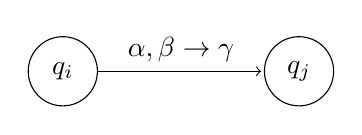
\begin{tikzpicture}[shorten >=1pt,node distance=3cm,on grid,auto]
\node[state] (q_i) {$q_i$};
\node[state] (q_j) [right=of q_i] {$q_j$};
\path[->]
(q_i) edge node {$\alpha,\beta \to \gamma$} (q_j);
\end{tikzpicture} \\
\end{minipage}


\HRule\\
First we denote our stack end as $\#$. Then we read a number of $x$'s and push them on the stack. Let's denote this number $k$. Now we have two choice, namely:\\
1) Read $k$ number of $y$'s and while we are reading $y$'s, we are popping the $x$'s. When we have the same number of $y$'s as $x$'s, we will see the bottom of the stack. We move to the $q_4$ as we are popping the bottom of the stack $\#$. Then we read arbitrary number of $z$'s.
\\
2) Read arbitrary number of $y$'s. Then, we move to $q_5$ ad start reading $z$'s, and while reading $z$'s we are popping $x$'s. When we see the bottom of the stack, and we have no input to read, we pop $\#$ and move to $q_6$ and finish reading.
\\
Thus, my answer is:\\
\begin{align*}
L&= (x^k y^k z^t) \cup (x^k y^t z^k),\ where\ t,k \geq 0\ ;\ t,k \in N
\end{align*}
\HRule\\


\paragraph{b)} 
Design a PDA to recognize language $ L=\{x^n y^{m+n} x^m \mid \; n,m \geq 0; \; n,m \in \mathbb{N}  \} $  \hfill \small{(5/30 pts)} \\

\HRule\\
\begin{center}
\begin{tikzpicture}[scale=0.2]
\tikzstyle{every node}+=[inner sep=0pt]
\draw [black] (10.3,-15.7) circle (3);
\draw (10.3,-15.7) node {$q_0$};
\draw [black] (34.6,-15.7) circle (3);
\draw (34.6,-15.7) node {$q_1$};
\draw [black] (60.2,-15.7) circle (3);
\draw (60.2,-15.7) node {$q_2$};
\draw [black] (60.2,-42.7) circle (3);
\draw (60.2,-42.7) node {$q_3$};
\draw [black] (10.3,-42.7) circle (3);
\draw (10.3,-42.7) node {$q_5$};
\draw [black] (10.3,-42.7) circle (2.4);
\draw [black] (34.6,-42.7) circle (3);
\draw (34.6,-42.7) node {$q_4$};
\draw [black] (13.3,-15.7) -- (31.6,-15.7);
\fill [black] (31.6,-15.7) -- (30.8,-15.2) -- (30.8,-16.2);
\draw (22.45,-16.2) node [below] {$e,e\mbox{ }\to\mbox{ }\#$};
\draw [black] (37.6,-15.7) -- (57.2,-15.7);
\fill [black] (57.2,-15.7) -- (56.4,-15.2) -- (56.4,-16.2);
\draw (47.4,-15.2) node [above] {$e,e,\mbox{ }\to\mbox{ }e$};
\draw [black] (60.2,-18.7) -- (60.2,-39.7);
\fill [black] (60.2,-39.7) -- (60.7,-38.9) -- (59.7,-38.9);
\draw (59.7,-29.2) node [left] {$e,e\mbox{ }\to\mbox{ }e$};
\draw [black] (57.2,-42.7) -- (37.6,-42.7);
\fill [black] (37.6,-42.7) -- (38.4,-43.2) -- (38.4,-42.2);
\draw (47.4,-42.2) node [above] {$e,e\mbox{ }\to\mbox{ }e$};
\draw [black] (31.6,-42.7) -- (13.3,-42.7);
\fill [black] (13.3,-42.7) -- (14.1,-43.2) -- (14.1,-42.2);
\draw (22.45,-42.2) node [above] {$e,\mbox{ }\#\mbox{ }\to\mbox{ }e$};
\draw [black] (33.277,-13.02) arc (234:-54:2.25);
\draw (34.6,-8.45) node [above] {$x,e\mbox{ }\to\mbox{ }x$};
\fill [black] (35.92,-13.02) -- (36.8,-12.67) -- (35.99,-12.08);
\draw [black] (61.06,-12.838) arc (191.00146:-96.99854:2.25);
\draw (68.5,-10.28) node [above] {$y,x\mbox{ }\to\mbox{ }e$};
\fill [black] (62.99,-14.64) -- (63.88,-14.98) -- (63.68,-14);
\draw [black] (63.179,-42.939) arc (113.14983:-174.85017:2.25);
\draw (66.64,-47.42) node [right] {$y,e\mbox{ }\to\mbox{ }y$};
\fill [black] (61.82,-45.21) -- (61.68,-46.14) -- (62.6,-45.75);
\draw [black] (35.923,-45.38) arc (54:-234:2.25);
\draw (34.6,-49.95) node [below] {$x,y\mbox{ }\to\mbox{ }e$};
\fill [black] (33.28,-45.38) -- (32.4,-45.73) -- (33.21,-46.32);
\end{tikzpicture}
\end{center}
Initial is $q_o$\\
First, mark the stack bottom.\\
Then, as we read $x$, push them on the stack.\\
While reading $y$'s, pop $x$'s that are on the stack.\\
When we reached to the bottom of the stack, start pushing $y$'s to the stack.\\
Again, while we are reading $x$'s, pop $y$'s that are on the stack.\\
When we have no input to read, and we have stack's bottom on the top of the stack, we can finish reading.\\
\HRule\\

\newpage

\paragraph{c)} 
Design a PDA to recognize language $ L=\{x^n y^m \mid \; n < m \leq 2n; \; n,m \in \mathbb{N^+} \} $  \hfill \small{(10/30 pts)} \\
Do not use multi-symbol push/pop operations in your transitions. \\
Simulate the PDA on strings \textit{xxy} (with only one rejecting derivation) and \textit{xxyyyy} (accepting derivation) with transition tables. \\


\HRule\\
\begin{center}
\begin{tikzpicture}[scale=0.2]
\tikzstyle{every node}+=[inner sep=0pt]
\draw [black] (4.8,-29.5) circle (3);
\draw (4.8,-29.5) node {$q_0$};
\draw [black] (24.3,-29.5) circle (3);
\draw (24.3,-29.5) node {$q_1$};
\draw [black] (48.8,-29.5) circle (3);
\draw (48.8,-29.5) node {$q_2$};
\draw [black] (51,-7.3) circle (3);
\draw (51,-7.3) node {$q_3$};
\draw [black] (51,-7.3) circle (2.4);
\draw [black] (70.2,-29.5) circle (3);
\draw (70.2,-29.5) node {$q_4$};
\draw [black] (7.8,-29.5) -- (21.3,-29.5);
\fill [black] (21.3,-29.5) -- (20.5,-29) -- (20.5,-30);
\draw (14.55,-30) node [below] {$e,e\mbox{ }\to\mbox{ }\#$};
\draw [black] (25.623,-32.18) arc (54:-234:2.25);
\draw (24.3,-36.75) node [below] {$x,e\mbox{ }\to\mbox{ }x$};
\fill [black] (22.98,-32.18) -- (22.1,-32.53) -- (22.91,-33.12);
\draw [black] (27.3,-29.5) -- (45.8,-29.5);
\fill [black] (45.8,-29.5) -- (45,-29) -- (45,-30);
\draw (36.55,-30) node [below] {$y,x\mbox{ }\to\mbox{ }x$};
\draw [black] (46.934,-27.158) arc (-147.35851:-223.96046:14.534);
\fill [black] (48.71,-9.23) -- (47.79,-9.46) -- (48.51,-10.15);
\draw (44.07,-17.8) node [left] {$e,\mbox{ }\#\mbox{ }\to\mbox{ }e$};
\draw [black] (67.778,-31.263) arc (-59.26084:-120.73916:16.195);
\fill [black] (67.78,-31.26) -- (66.83,-31.24) -- (67.35,-32.1);
\draw (59.5,-34.04) node [below] {$y,x\mbox{ }\to\mbox{ }e$};
\draw [black] (50.384,-32.034) arc (59.74518:-228.25482:2.25);
\draw (50.18,-37.02) node [below] {$y,x\mbox{ }\to\mbox{ }e$};
\fill [black] (47.75,-32.3) -- (46.92,-32.74) -- (47.78,-33.24);
\draw [black] (51.036,-27.508) arc (125.76275:54.23725:14.482);
\fill [black] (51.04,-27.51) -- (51.98,-27.45) -- (51.39,-26.63);
\draw (59.5,-24.28) node [above] {$y,x\mbox{ }\to\mbox{ }x$};
\end{tikzpicture}
\end{center}
Initial state is $q_0$.\\
First, we mark the bottom of the stack.\\
Then, we are pushing $x$'s to the stack.\\
When we encounter with a $y$, we don't immediately pop a $x$. We move to $q_2$.\\
When we are reading $y$'s, we either pop an $x$ and stay at $q_2$ or we move to $q_4$ while popping a $x$.\\
If we are at $q_4$, we are checking the stack to make our move, because if we don't have a $x$ on the stack, that means we have 2 times more $y$'s than $x$'s.\\
While at $q_2$, if we don't have any input to read and our top of the stack is $\#$, we move to $q_3$ and terminate the reading process.\\
The simulation for $xxy$ is:
\begin{table}[H]
\centering
\begin{tabular}{lll}
State & Unread Input & Stack \\
q0    & xxy          & e     \\
q1    & xxy          & \#    \\
q1    & xy           & x\#   \\
q1    & y            & xx\#  \\
q2    & e            & xx\# 
\end{tabular}
\end{table}
Rejected.\\
The simulation for $xxyyyy$ is:\\
\begin{table}[H]
\centering
\begin{tabular}{lll}
State & Unread Input & Stack \\
q0    & xxyyyy       & e     \\
q1    & xxyyyy       & \#    \\
q1    & xyyyy        & x\#   \\
q1    & yyyy         & xx\#  \\
q2    & yyy          & xx\#  \\
q4    & yy           & x\#   \\
q2    & y            & x\#   \\
q2    & e            & \#    \\
q3    &              &      
\end{tabular}
\end{table}
Accepted.\\
\HRule\\

\paragraph{d)} Given two languages $L'$ and $L$ as $L'=\{w \mid \; w\in L; \; |w|=4n+2 \; for\; n\in \mathbb{N} \}$
\hfill \small{(10/30 pts)} \\
If $L$ is a CFL, show that $L'$ is also a CFL by constructing an automaton for $L'$ in terms of another automaton that recognizes $L$. \\

\HRule\\
Assume that the construction of such L is given. Also, we can draw an automata for $L_2$ such that it accepts the same language as $L'$ accepts.
\begin{center}
\begin{tikzpicture}[scale=0.2]
\tikzstyle{every node}+=[inner sep=0pt]
\draw [black] (10.3,-22) circle (3);
\draw (10.3,-22) node {$q_0$};
\draw [black] (27.1,-22) circle (3);
\draw (27.1,-22) node {$q_1$};
\draw [black] (44.6,-22) circle (3);
\draw (44.6,-22) node {$q_2$};
\draw [black] (62.1,-22) circle (3);
\draw (62.1,-22) node {$q_3$};
\draw [black] (10.3,-43.5) circle (3);
\draw (10.3,-43.5) node {$q_4$};
\draw [black] (36.2,-43.5) circle (3);
\draw (36.2,-43.5) node {$q_5$};
\draw [black] (36.2,-43.5) circle (2.4);
\draw [black] (13.3,-22) -- (24.1,-22);
\fill [black] (24.1,-22) -- (23.3,-21.5) -- (23.3,-22.5);
\draw [black] (30.1,-22) -- (41.6,-22);
\fill [black] (41.6,-22) -- (40.8,-21.5) -- (40.8,-22.5);
\draw [black] (47.6,-22) -- (59.1,-22);
\fill [black] (59.1,-22) -- (58.3,-21.5) -- (58.3,-22.5);
\draw [black] (12.538,-20.004) arc (129.42283:50.57717:37.26);
\fill [black] (12.54,-20) -- (13.47,-19.88) -- (12.84,-19.11);
\draw [black] (10.3,-25) -- (10.3,-40.5);
\fill [black] (10.3,-40.5) -- (10.8,-39.7) -- (9.8,-39.7);
\draw [black] (13.3,-43.5) -- (33.2,-43.5);
\fill [black] (33.2,-43.5) -- (32.4,-43) -- (32.4,-44);
\end{tikzpicture}
\end{center}
Where $q_0$ is initial and there is a input reading between those states.\\ Since $L_2$ is a regular language, because I have drawn the automata for that, using the Theorem 3.5.2 in the book, the intersection of a CFL and Regular Language is a CFL, we can create the following:
\begin{align*}
L' = L \cap L_2
\end{align*}
such that, we have a stack to keep tabs on the stack of $L'$, the initial and final states of this language are from both $L'$ and $L_2$'s accepting states, and the states of this language are pair of $L'$ and $L_2$'s states.\\
\HRule\\

\newpage
\section{Closure Properties \hfill \normalfont{(20 pts)}}

Let $L_1$ and $L_2$ be context-free languages which are not regular, and let $L_3$ be a regular language. Determine whether the following languages are necessarily CFLs or not. If they need to be context-free, explain your reasoning. If not, give one example where the language is a CFL and a counter example where the language is not a CFL. \\

\paragraph{a)} $L_4 = L_1 \cap (L_2 \setminus L_3)$ \hfill \small{(10/20 pts)} \\

\HRule\\
Let $L_2$ and $L_3$ denotes the following:\\
\begin{align*}
L_2&= (a^n b^n c^m d^m),\ where\ m,n \geq 1 \\
L_3&= (a \cup b)^* \\
\end{align*}
Thus, $L_2$ is context free but not regular, and $L_3$ is a regular language, as in stated in the question.
\begin{align*}
L_2 \setminus L_3&= L_2 \\
\end{align*}
And the intersection of two context free language is unknown because context free languages are not closed under intersection. Hence, we cannot know whether the $L_4$ context free or not.\\
\HRule\\

\paragraph{b)} $L_5 = (L_1 \cap L_3)\text{*}$ \hfill \small{(10/20 pts)} \\

\HRule\\
Let a PDA named $P$ accepts $L_1$, and let a DFA named $M$ accepts $L_3$. We can create a new PDA that simulate $P$ and $M$ at the same time on the same input, and accept if both of them accepts. Then this new PDA can accept $L_1$ and $L_3$'s intersection. Since context free languages are closed under Kleene star operation, $L_5$ is a context free language. Constructing this new PDA's algorithm is:\\
The stack of new PDA is the stack of $P$\\
The state of this new PDA is te pair of states of $P$ and $M$ \\
These can determine the transition function of this new PDA \\
And the final states of this new PDA are $P$'s and $M$'s accepting states \\
\href{https://courses.engr.illinois.edu/cs373/fa2010/Lectures/notes25.pdf}{Reference} \\
\HRule\\

\newpage
\section{Pumping Theorem \hfill \normalfont{(20 pts)}}

\paragraph{a)} Show that $L=\{a^n m^n t^i \mid \; n\leq i \leq 2n\}$ is not a Context Free Language \hfill \small{(10/20 pts)} \\
using Pumping Theorem for CFLs. \\

\HRule\\
Suppose we have $S$, where $S$ is in form of $uv^nxy^nz$ and $n \geq 0$.\\
Then, we should have;\\
$uv^ixy^iz$ for every $i \geq 0$, $|vy| > 0$, and $|vxy| \leq P$, where $P$ denotes pumping length.\\
We will have 4 cases, where each is the following:\\\\
$i)$ We have at least one $t$ in substring and along with $t$('s), we have $m$('s).\\
$ii)$We only have at least one $t$ in substring.$\#t \geq 1$ \\
$iii)$We don't have $t$'s in substring. Then we have either at least one $a$'s or at least one $m$'s in this substring. Not both of them.\\
$iv)$We don't have $t$'s in substring. But we have both at least one $a$'s and $m$'s in the substring.\\
\\

$i)$Assume the first case: we have at least one $t$ along with $m$'s in this substring $vxy$.\\
Then, if we use pump, the number of $a$'s and $m$'s will not be equal, because if we have $t$, then we don't have any $a$ along with those $m$'s, because the length of substring $xvy$ must be less than our pumping length. Therefore it is a contradiction in this case.\\\\
$ii)$Assume the second case: we have only at least one $t$.\\
Then, if we pump $i > P$, the second restriction will not be held ($i \leq 2n$).\\
For clarification:\\
we have aaammmttt. If we choose our substring as a $t$, and if we pump 4 times, which is greater than 3($\#P$), then we will have more than $2n$ $t$'s. If I have choosen to write more than 3 $t$'s in the example, i.e. 4-5-6, then the number of $i$ will be decreased. But $i > P$ holds for every $P$ regardless of the input.\\
Therefore it is a cntradiction in this case.\\\\
$iii)$Assume the third case: We don't have $t$'s in the substring. We have $a$'s or $m$'s, but not both. Then, it is easy to see that if we pump one of them, the equation of their length will not be true. Therefore we cannot accept this state either.\\\\
$iv)$Assume the forth and the last case: We don't have $t$'s in the substring, but we have $a$'s and $m$'s together.\\
As in stated in the second case, if we pump this substring more than $P$ time, $i > P$, the second restriction will not be held.\\
For clarification:\\
We have aaammmttttttt. We choose our substring as $am$. Our pumping length is 3. If we pump this substring 4 times, more than 3 times, we will have more than 7 $a$'s and $b$'s, but we have at most 6 $t$'s at the first step.\\\\
Since all the cases above are contradiction, this language is not a CFL.\\
\HRule\\


\paragraph{b)} Show that $L=\{a^n b^{2n} a^n \mid \; n \in \mathbb{N+} \}$ is not a Context Free Language \hfill \small{(10/20 pts)} \\
using Pumping Theorem for CFLs. \\

\HRule\\
Suppose we have $S$, where $S$ is in form of $uv^nxy^nz$ and $n \geq 0$.\\
Then, we should have;\\
$uv^ixy^iz$ for every $i \geq 0$, $|vy| > 0$, and $|vxy| \leq P$, where $P$ denotes pumping length.\\
Assume that we have only $a$'s in this substring $vxy$. Then with any $i \geq 0$, we have an imbalance between $a$'s and $b$'s. Therefore our substring cannot contain only $a$'s.\\
Which brings us to the second case, where our substring contains both $a$'s and $b$'s. To avoid imbalance, we should have a number of $a$'s, then a number of $b$'s and at last, a number of $a$'s again. However, since our substring is continous, it should contain all $b$'s in order to connect both $a$'s in different sides. i.e. oursubstring is in this form:
\begin{align*}
aaa...aaabbb...bbbbaaa....a
\end{align*} 
In this form, we don't have any relation of number of $a$'s in the left of $b$'s and the number of $a$'s in the right of the $b$'s. Also we do not have the rule for number of $a$'s is half of the number of $b$'s for each side. One can see that, to obtain such substring, we need to have all  $b$'s. Since our pumping length is $P$, and the number of $b$'s is $2P$, we have a contradiction in $|vxy| \leq P$, therefore we cannot have this kind of string either.\\
The third case is, our substring can contain only $b$'s. It is easy to see that it will cause an imbalance between the number of $a$'s and the number of $b$'s, because when $i$ increases, only the number of $b$'s increases, and we won't have the equality for each $i$.\\
All in all, all cases that don't contain all $b$'s break symmetry, and the case that contains all $b$'s is not applicable, because it contradicts with the pumping lemma. Therefore, we cannot have this string in our language.\\
\HRule\\





\newpage
\section{CNF and CYK \hfill \normalfont{(not graded)}}

\paragraph{a)} Convert the given context-free grammar to Chomsky Normal Form. \\

$ S   \to XSX \mid xY $ \\
$ X   \to Y \mid S $ \\
$ Y   \to z \mid \varepsilon $ \\

\begin{tcolorbox}
answer here ...
\vspace{18cm} % remove this after your answer
\end{tcolorbox}


\paragraph{b)} Use the grammar below to parse the given sentence using Cocke–Younger–Kasami algorithm. \\
Plot the parse trees. \\

\begin{multicols}{2}
S $\to$ NP VP \\
S $\to$ X1 VP \\
X1 $\to$ Aux NP \\
S $\to$ book $\mid$ include $\mid$ prefer \\
S $\to$ Verb NP \\
S $\to$ X2 PP \\
S $\to$ Verb PP \\
S $\to$ VP PP \\
NP $\to$ I $\mid$ she $\mid$ me $\mid$ Houston \\
NP $\to$ Det Nom \\
Nom $\to$ book $\mid$ flight $\mid$ meal $\mid$ money \\
Nom $\to$ Nom Noun \\
Nom $\to$ Nom PP \\
VP $\to$ book $\mid$ include $\mid$ prefer \\
VP $\to$ Verb NP \\
VP $\to$ X2 PP \\
X2 $\to$ Verb NP \\
VP $\to$ Verb PP \\
VP $\to$ VP PP \\
PP $\to$ Prep NP \\
Det $\to$ that $\mid$ this $\mid$ the $\mid$ a \\
Noun $\to$ book $\mid$ flight $\mid$ meal $\mid$ money \\
Verb $\to$ book $\mid$ include $\mid$ prefer \\
Aux $\to$ does \\
Prep $\to$ from $\mid$ to $\mid$ on $\mid$ near $\mid$ through \\
\end{multicols}

\vspace{5mm}

book the flight through Houston \\

\begin{tcolorbox}

\scriptsize

Empty parse table:\\
\begin{tikzpicture}[node distance=0cm, outer sep = 0pt]

\node[terminal] (l0) {
    \begin{tabular}{@{}P{2.9cm}|@{}P{2.9cm}|@{}P{2.9cm}|@{}P{2.9cm}|@{}P{2.9cm}}
    book & the & flight & through & Houston \\
    \end{tabular}
};

\node[nonterminal] (l1) [above = of l0] {
    \begin{tabular}{@{}P{2.9cm}|@{}P{2.9cm}|@{}P{2.9cm}|@{}P{2.9cm}|@{}P{2.9cm}}
    1:1 & 
    2:2 & 
    3:3 & 
    4:4 & 
    5:5 \\
    \end{tabular}
};

\node[nonterminal] (l2) [above = of l1.north] {
    \begin{tabular}{@{}P{2.9cm}|@{}P{2.9cm}|@{}P{2.9cm}|@{}P{2.9cm}}
    1:2 $\to$ 1:1 2:2 & 
    2:3 $\to$ 2:2 3:3 & 
    3:4 $\to$ 3:3 4:4 & 
    4:5 $\to$ 4:4 5:5 \\
    \end{tabular}
};

\node[nonterminal] (l3) [above = of l2.north] {
    \begin{tabular}{@{}P{2.9cm}|@{}P{2.9cm}|@{}P{2.9cm}}
        \begin{tabular}{@{}l} 1:3 $\to$ 1:1 2:3 \\ 1:3 $\to$ 1:2 3:3 \end{tabular}& 
        \begin{tabular}{@{}l} 2:4 $\to$ 2:2 3:4 \\ 2:4 $\to$ 2:3 4:4 \end{tabular}& 
        \begin{tabular}{@{}l} 3:5 $\to$ 3:3 4:5 \\ 3:5 $\to$ 3:4 5:5 \end{tabular}\\
    \end{tabular}
};

\node[nonterminal] (l4) [above = of l3.north] {
    \begin{tabular}{@{}P{2.9cm}|@{}P{2.9cm}}
        \begin{tabular}{@{}l}1:4 $\to$ 1:1 2:4 \\ 1:4 $\to$ 1:2 3:4 \\ 1:4 $\to$ 1:3 4:4 \end{tabular}& 
        \begin{tabular}{@{}l}2:5 $\to$ 2:2 3:5 \\ 2:5 $\to$ 2:3 4:5 \\ 2:5 $\to$ 2:4 5:5 \end{tabular}\\
    \end{tabular}
};

\node[nonterminal] (l5) [above = of l4.north] {
    \begin{tabular}{@{}P{2.9cm}}
        \begin{tabular}{@{}l}
        1:5 $\to$ 1:1 2:5 \\ 1:5 $\to$ 1:2 3:5 \\ 
        1:5 $\to$ 1:3 4:5 \\ 1:5 $\to$ 1:4 5:5 
        \end{tabular}\\
    \end{tabular}
};

\end{tikzpicture}\\\\

rest of the answer here ...\\
\vspace{4cm} % remove this after your answer
\end{tcolorbox}



\newpage
\section{Deterministic Pushdown Automata \hfill \normalfont{(not graded)}}
Provide a DPDA to recognize the given languages, the DPDA must read its entire input and finish with an empty stack.
\paragraph{a)} $a^*bc \cup a^nb^nc$ \\

\begin{tcolorbox}
answer here ...
\vspace{12cm} % remove this after your answer
\end{tcolorbox}

\newpage

\paragraph{b)} $(aa)^*c \cup a^nb^nc$ \\

\begin{tcolorbox}
answer here ...
\vspace{12cm} % remove this after your answer
\end{tcolorbox}



\end{document}

​
